\documentclass[a4paper,12pt,twoside]{memoir}

% Castellano
\usepackage[spanish,es-tabla]{babel}
\selectlanguage{spanish}
\usepackage[utf8]{inputenc}
\usepackage[T1]{fontenc}
\usepackage{lmodern} % Scalable font
\usepackage{microtype}
\usepackage{placeins}
\usepackage[official]{eurosym}

\RequirePackage{booktabs}
\RequirePackage[table]{xcolor}
\RequirePackage{xtab}
\RequirePackage{multirow}

% Links
\usepackage[colorlinks]{hyperref}
\hypersetup{
	allcolors = {red}
}

% Ecuaciones
\usepackage{amsmath}

% Rutas de fichero / paquete
\newcommand{\ruta}[1]{{\sffamily #1}}

% Párrafos
\nonzeroparskip


% Imagenes
\usepackage{graphicx}
\newcommand{\imagen}[2]{
	\begin{figure}[!h]
		\centering
		\includegraphics[width=0.9\textwidth]{#1}
		\caption{#2}\label{fig:#1}
	\end{figure}
	\FloatBarrier
}

\newcommand{\imagenflotante}[2]{
	\begin{figure}%[!h]
		\centering
		\includegraphics[width=0.9\textwidth]{#1}
		\caption{#2}\label{fig:#1}
	\end{figure}
}



% El comando \figura nos permite insertar figuras comodamente, y utilizando
% siempre el mismo formato. Los parametros son:
% 1 -> Porcentaje del ancho de página que ocupará la figura (de 0 a 1)
% 2 --> Fichero de la imagen
% 3 --> Texto a pie de imagen
% 4 --> Etiqueta (label) para referencias
% 5 --> Opciones que queramos pasarle al \includegraphics
% 6 --> Opciones de posicionamiento a pasarle a \begin{figure}
\newcommand{\figuraConPosicion}[6]{%
  \setlength{\anchoFloat}{#1\textwidth}%
  \addtolength{\anchoFloat}{-4\fboxsep}%
  \setlength{\anchoFigura}{\anchoFloat}%
  \begin{figure}[#6]
    \begin{center}%
      \Ovalbox{%
        \begin{minipage}{\anchoFloat}%
          \begin{center}%
            \includegraphics[width=\anchoFigura,#5]{#2}%
            \caption{#3}%
            \label{#4}%
          \end{center}%
        \end{minipage}
      }%
    \end{center}%
  \end{figure}%
}

%
% Comando para incluir imágenes en formato apaisado (sin marco).
\newcommand{\figuraApaisadaSinMarco}[5]{%
  \begin{figure}%
    \begin{center}%
    \includegraphics[angle=90,height=#1\textheight,#5]{#2}%
    \caption{#3}%
    \label{#4}%
    \end{center}%
  \end{figure}%
}
% Para las tablas
\newcommand{\otoprule}{\midrule [\heavyrulewidth]}
%
% Nuevo comando para tablas pequeñas (menos de una página).
\newcommand{\tablaSmall}[5]{%
 \begin{table}
  \begin{center}
   \rowcolors {2}{gray!35}{}
   \begin{tabular}{#2}
    \toprule
    #4
    \otoprule
    #5
    \bottomrule
   \end{tabular}
   \caption{#1}
   \label{tabla:#3}
  \end{center}
 \end{table}
}

%
% Nuevo comando para tablas pequeñas (menos de una página).
\newcommand{\tablaSmallSinColores}[5]{%
 \begin{table}[H]
  \begin{center}
   \begin{tabular}{#2}
    \toprule
    #4
    \otoprule
    #5
    \bottomrule
   \end{tabular}
   \caption{#1}
   \label{tabla:#3}
  \end{center}
 \end{table}
}

\newcommand{\tablaApaisadaSmall}[5]{%
\begin{landscape}
  \begin{table}
   \begin{center}
    \rowcolors {2}{gray!35}{}
    \begin{tabular}{#2}
     \toprule
     #4
     \otoprule
     #5
     \bottomrule
    \end{tabular}
    \caption{#1}
    \label{tabla:#3}
   \end{center}
  \end{table}
\end{landscape}
}

%
% Nuevo comando para tablas grandes con cabecera y filas alternas coloreadas en gris.
\newcommand{\tabla}[6]{%
  \begin{center}
    \tablefirsthead{
      \toprule
      #5
      \otoprule
    }
    \tablehead{
      \multicolumn{#3}{l}{\small\sl continúa desde la página anterior}\\
      \toprule
      #5
      \otoprule
    }
    \tabletail{
      \hline
      \multicolumn{#3}{r}{\small\sl continúa en la página siguiente}\\
    }
    \tablelasttail{
      \hline
    }
    \bottomcaption{#1}
    \rowcolors {2}{gray!35}{}
    \begin{xtabular}{#2}
      #6
      \bottomrule
    \end{xtabular}
    \label{tabla:#4}
  \end{center}
}

%
% Nuevo comando para tablas grandes con cabecera.
\newcommand{\tablaSinColores}[6]{%
  \begin{center}
    \tablefirsthead{
      \toprule
      #5
      \otoprule
    }
    \tablehead{
      \multicolumn{#3}{l}{\small\sl continúa desde la página anterior}\\
      \toprule
      #5
      \otoprule
    }
    \tabletail{
      \hline
      \multicolumn{#3}{r}{\small\sl continúa en la página siguiente}\\
    }
    \tablelasttail{
      \hline
    }
    \bottomcaption{#1}
    \begin{xtabular}{#2}
      #6
      \bottomrule
    \end{xtabular}
    \label{tabla:#4}
  \end{center}
}

%
% Nuevo comando para tablas grandes sin cabecera.
\newcommand{\tablaSinCabecera}[5]{%
  \begin{center}
    \tablefirsthead{
      \toprule
    }
    \tablehead{
      \multicolumn{#3}{l}{\small\sl continúa desde la página anterior}\\
      \hline
    }
    \tabletail{
      \hline
      \multicolumn{#3}{r}{\small\sl continúa en la página siguiente}\\
    }
    \tablelasttail{
      \hline
    }
    \bottomcaption{#1}
  \begin{xtabular}{#2}
    #5
   \bottomrule
  \end{xtabular}
  \label{tabla:#4}
  \end{center}
}



\definecolor{cgoLight}{HTML}{EEEEEE}
\definecolor{cgoExtralight}{HTML}{FFFFFF}

%
% Nuevo comando para tablas grandes sin cabecera.
\newcommand{\tablaSinCabeceraConBandas}[5]{%
  \begin{center}
    \tablefirsthead{
      \toprule
    }
    \tablehead{
      \multicolumn{#3}{l}{\small\sl continúa desde la página anterior}\\
      \hline
    }
    \tabletail{
      \hline
      \multicolumn{#3}{r}{\small\sl continúa en la página siguiente}\\
    }
    \tablelasttail{
      \hline
    }
    \bottomcaption{#1}
    \rowcolors[]{1}{cgoExtralight}{cgoLight}

  \begin{xtabular}{#2}
    #5
   \bottomrule
  \end{xtabular}
  \label{tabla:#4}
  \end{center}
}


















\graphicspath{ {./img/} }

% Capítulos
\chapterstyle{bianchi}
\newcommand{\capitulo}[2]{
	\setcounter{chapter}{#1}
	\setcounter{section}{0}
	\chapter*{#2}
	\addcontentsline{toc}{chapter}{#2}
	\markboth{#2}{#2}
}

% Apéndices
\renewcommand{\appendixname}{Apéndice}
\renewcommand*\cftappendixname{\appendixname}

\newcommand{\apendice}[1]{
	%\renewcommand{\thechapter}{A}
	\chapter{#1}
}

\renewcommand*\cftappendixname{\appendixname\ }

% Formato de portada
\makeatletter
\usepackage{xcolor}
\newcommand{\tutor}[1]{\def\@tutor{#1}}
\newcommand{\course}[1]{\def\@course{#1}}
\definecolor{cpardoBox}{HTML}{E6E6FF}
\def\maketitle{
  \null
  \thispagestyle{empty}
  % Cabecera ----------------
\noindent
\includegraphics[width=\textwidth]{cabecera}\vspace{1cm}%
  \vfill
  % Título proyecto y escudo informática ----------------
  \colorbox{cpardoBox}{%
    \begin{minipage}{.8\textwidth}
      \vspace{.5cm}\Large
      \begin{center}
      \textbf{TFG del Grado en Ingeniería Informática}\vspace{.6cm}\\
      \textbf{\LARGE\@title{}}
      \end{center}
      \vspace{.2cm}
    \end{minipage}

  }%
  \hfill\begin{minipage}{.20\textwidth}
    
\includegraphics[width=\textwidth]{escudoInfor}
  \end{minipage}
  \vfill
  % Datos de alumno, curso y tutores ------------------
  \begin{center}%
  {%
    \noindent\LARGE
    Presentado por \@author{}\\ 
    en Universidad de Burgos --- \@date{}\\
    Tutores: \@tutor{}\\
  }%
  \end{center}%
  \null
  \cleardoublepage
  }
\makeatother

\newcommand{\nombre}{Zoe Calvo Serna} %%% cambio de comando

% Datos de portada
\title{Sentinel}
\author{\nombre}
\tutor{José Manuel Galán Ordax y Virginia Ahedo García}
\date{\today}

\begin{document}

\maketitle


\newpage\null\thispagestyle{empty}\newpage


%%%%%%%%%%%%%%%%%%%%%%%%%%%%%%%%%%%%%%%%%%%%%%%%%%%%%%%%%%%%%%%%%%%%%%%%%%%%%%%%%%%%%%%%
\thispagestyle{empty}


\noindent
\includegraphics[width=\textwidth]{cabecera}\vspace{1cm}

\noindent D. José Manuel Galán Ordax y Dª Virginia Ahedo García, profesores del departamento de Ingeniería Civil, área de Ingeniería de Organización.

\noindent Expone:

\noindent Que el alumno D. \nombre, con DNI 71309260Z, ha realizado el Trabajo final de Grado en Ingeniería Informática titulado Sentinel. 

\noindent Y que dicho trabajo ha sido realizado por el alumno bajo la dirección del que suscribe, en virtud de lo cual se autoriza su presentación y defensa.

\begin{center} %\large
En Burgos, {\large \today}
\end{center}

\vfill\vfill\vfill

% Author and supervisor
\begin{minipage}{0.45\textwidth}
\begin{flushleft} %\large
Vº. Bº. del Tutor:\\[2cm]
D. José Manuel Galán Ordax
\end{flushleft}
\end{minipage}
\hfill
\begin{minipage}{0.45\textwidth}
\begin{flushleft} %\large
Vº. Bº. del co-tutor:\\[2cm]
Dª. Virginia Ahedo García
\end{flushleft}
\end{minipage}
\hfill

\vfill

% para casos con solo un tutor comentar lo anterior
% y descomentar lo siguiente
%Vº. Bº. del Tutor:\\[2cm]
%D. nombre tutor


\newpage\null\thispagestyle{empty}\newpage




\frontmatter

% Abstract en castellano
\renewcommand*\abstractname{Resumen}
\begin{abstract}
Este proyecto utilizará las APIs de las redes sociales principales (instagram, twitter,...) para crear una aplicación que permita estudiar mediante sentiment analysis las series temporales de percepción de diferentes marcas comerciales, procesos sociológicos, el efecto de campañas de marketing, etc.
\end{abstract}

\renewcommand*\abstractname{Descriptores}
\begin{abstract}
Sentiment analysis, redes sociales, twitter, instagram, servidor flask, aplicación web, angular, rest. 
\end{abstract}

\clearpage

% Abstract en inglés
\renewcommand*\abstractname{Abstract}
\begin{abstract}
This project will use the APIs of the main social networks (instagram, twitter,...) to create an application that allows you to study through sentiment analysis the time series of different trademarks, sociological processes, the effect of marketing campaigns...
\end{abstract}

\renewcommand*\abstractname{Keywords}
\begin{abstract}
Sentiment analysis, social networks, twitter, instagram, flask server, web application, angular, rest.
\end{abstract}

\clearpage

% Indices
\tableofcontents

\clearpage

\listoffigures

\clearpage

\listoftables
\clearpage

\mainmatter
\capitulo{1}{Introducción}

Un pilar básico en las organizaciones públicas y privadas que se dirigen a la sociedad, ya sea ofreciendo un producto o un servicio, es la opinión de las personas. 

En el pasado la forma de conocer estas opiniones era mediante encuestas que después se trataban para hacer estadísticas y evaluar la calidad del producto.

Estas encuestas tiene dos grandes limitaciones:
\begin{itemize}
\tightlist
    \item La muestra es limitada y a partir de esta debemos generalizar.
    \item La opinión de esta población viene dada por unas preguntas que realiza la organización previamente, por tanto son demasiado específicas y puede que haya aspectos que no se tengan en cuenta.
\end{itemize}

Hoy en día las redes sociales constituyen un gran avance en este ámbito. La gente puede mostrar su opinión sobre cualquier servicio o producto sin necesidad de encuestas y además pueden tener un alcance global.
Esto representa un gran cambio tanto para las personas como para las organizaciones. La gente puede basarse en la opinión de personas muy dispares para tomar decisiones sobre un producto. Las organizaciones pueden aprovecharse de la diversidad de la población y de la sinceridad de la opinión ya que no está acotada por preguntas exactas.

En este punto es donde el análisis de sentimiento toma protagonismo. Este concepto no es más que el estudio del lenguaje natural, análisis de texto y lingüística computacional, para tratar de establecer métricas capaces de capturar el sentimiento general de un texto. 

Es un campo muy grande que abarca diferentes técnicas. Como ocurre con otros términos, es más conocido el nombre en inglés, Sentiment Analysis, por lo que a partir de ahora nos referiremos al tema con el término anglosajón.

Estas métricas han hecho que las organizaciones complementen sus encuestas con los resultados obtenidos en las redes sociales y así poder tener un mayor feedback sobre sus servicios. 

En este trabajo se propone la utilización de Sentiment Analysis para realizar estudios en Twitter e Instagram sobre temas de actualidad, productos o servicios. 
Para ello se recopilará información de estas redes sociales y se mostrará en gráficos y tablas para hacer más fácil la interpretación de los datos.



\section{Estructura de la memoria}
\begin{itemize}
\tightlist
    \item
        \textbf{Introducción: }Descripción de la situación y el tema sobre el que el proyecto va a versar. Estructura de la memoria y de los anexos.
    \item 
        \textbf{Objetivos del proyecto: }Explicación de los temas a tratar en el trabajo.
    \item 
        \textbf{Conceptos teóricos: }Exposición de conceptos que facilitan la comprensión del proyecto.
    \item 
        \textbf{Técnicas y herramientas: }Listado de metodologías y herramientas que han sido utilizadas para llevar a cabo el proyecto. 
    \item 
        \textbf{Aspectos relevantes: }Muestra aspectos a destacar durante la realización del proyecto
    \item 
        \textbf{Trabajos relacionados: }Estado del arte en el ámbito del sentiment analysis y trabajos similares.
    \item 
        \textbf{Conclusiones y líneas de trabajo futuras: }Conclusiones obtenidas al final del proyecto y posibles ideas futuras.
\end{itemize}

\newpage
\section{Estructura de los anexos}
\begin{itemize}
\tightlist
    \item 
        \textbf{Plan de proyecto software: }Planificación temporal y viabilidad económica y legal.
    \item 
        \textbf{Especificación de requisitos: }Objetivos y y requisitos establecidos al comienzo del proyecto.
    \item 
        \textbf{Especificación de diseño: }Recoge los diseños de datos, procedimental, arquitectónico y de interfaces.
    \item 
        \textbf{Manual del programador: }Explica los conceptos más técnicos del proyecto como su instalación, la organización de carpetas y la ejecución.
    \item 
        \textbf{Manual de usuario: }Es la guía de cómo utilizar la aplicación paso a paso.
\end{itemize}
\capitulo{2}{Objetivos del proyecto}

En este apartado vamos a detallar los objetivos que queremos abordar en el proyecto, que serán denominados generales, y los objetivos necesarios para llevar a cabo los anteriores, que denominaremos como técnicos.

\section{Objetivos generales}
\begin{itemize}
\tightlist
    \item Extraer datos de las redes sociales Twitter e Instagram.
    \item Estudiar mediante Sentiment Analysis la información recogida de estas APIs.
    \item Realizar estadísticas sobre los datos recopilados.
    \item Crear una aplicación web para mostrar la información.
    \item Mostrar las estadísticas mediante gráficos y tablas.
    \item Analizar mediante series temporales tendencias futuras en la evolución de las métricas.
    \item Crear una wiki para el manual de usuario.
\end{itemize}

\clearpage

\section{Objetivos técnicos}
\begin{itemize}
\tightlist
    \item Extraer los datos de las APIs de Twitter e Instagram.
    \item Utilizar librerías de Sentiment Analysis para analizar los datos obtenidos.
    \item Realizar operaciones estadísticas sobre los resultados de Sentiment Analysis.
    \item Almacenar en la base de datos los datos de las APIs junto a sus resultados y cálculos de las operaciones estadísticas.
    \item Desarrollar una interfaz que sea adaptativa y fácil de utilizar para el usuario.
    \item La aplicación deberá mostrar los resultados en gráficos y tablas.
    \item Utilizar Git como sistema de control de versiones junto con la plataforma GitHub.
    \item Usar la plataforma gráfica GitKraken para Git.
    \item Hacer uso de ZenHub para la gestión del proyecto.
    \item Utilizar un sistema para las referencias bibliográficas como Zotero.
    \item Utilizar la librería statsmodels de Python para calcular series temporales y realizar test para ver si es estacionaria.
\end{itemize}
\capitulo{3}{Conceptos teóricos}

\section{Sentiment Analysis}
El análisis de sentimiento \cite{sentiment_analysis} es una disciplina informática que se basa en identificar de forma automática las opiniones, sentimientos, pensamientos y emociones de las personas a través de textos, vídeos o audios. Esta rama de estudio pertenece al ámbito de la inteligencia artificial, ciencia social y ciencias de la computación.
El análisis de sentimiento puede aplicarse a diferentes niveles:
\begin{itemize}
\tightlist
    \item Detección de subjetividad: Solamente distingue entre si un comentario es subjetivo u objetivo.
    \item Detección de polaridad: Tras detectar que el comentario es subjetivo, determina si es positivo o negativo.
\end{itemize}

El interés de esta disciplina es que puede usarse tanto a nivel de aplicaciones destinadas a empresas y en redes sociales, pero también puede aplicarse a la educación y al cuidado de la salud.

Existen tres métodos aplicables para extraer la polaridad de un texto:
\begin{itemize}
\tightlist
    \item Método basado en la lingüística: Se asocia un valor real a cada concepto que se extrae de la frase. Luego se corrigen y se combinan todos en un solo valor. En el proceso de combinación el valor irá cambiando dependiendo de palabras como 'pero' o 'muy'.
    \item Método basado en machine learning: Se utiliza una máquina la cual extrae los conceptos de la frase en un vector y les aplica un algoritmo de forma automática para generar el valor de la polaridad.
    \item Método combinado: Se basa en combinar las dos técnicas anteriores. Puede ocurrir que la primera técnica no consiga extraer la polaridad, pero sus resultados son más fiables. Por ello, en la combinación la técnica de machine learning respalda a la de lingüística para ofrecer los mejores resultados.
\end{itemize}

\section{API}
Una API \cite{api} es un conjunto de código utilizado para desarrollar el software de aplicaciones. 
Las siglas se refieren a Application Programming Interface o Interfaz de Programación de Aplicaciones.

Son clave para la simplificación del desarrollo de aplicaciones, ya que no es necesario conocer la implementación de sus productos para poder comunicarse con ellos. 

Otras ventajas importantes son:
\begin{itemize}
\tightlist
    \item Dan flexibilidad.
    \item Simplifican el diseño y el uso de la aplicación.
    \item Ahorran tiempo y dinero.
\end{itemize}

\section{Web Service}
Un web service \cite{web_service} es un conjunto de protocolos y estándares que es utilizado por aplicaciones que están escritas en distintos lenguajes de programación para intercambiar información entre ellas.
Estas aplicaciones envían parámetros al servidor donde se aloja el web service y este les responde la petición.

Algunas de las mejoras que aportan a las aplicaciones son las siguientes:
\begin{itemize}
\tightlist
    \item Proporcionan interoperabilidad entre aplicaciones software, sin importar la plataforma sobre la que estén instaladas.
    \item Permite que los servicios de una compañía se comuniquen con los de otra que está en diferente lugar geográfico.
    \item Se aprovecha de los sistemas de seguridad firewall del protocolo HTTP.
    \item Fomentan la utilización de estándares y protocolos basados en texto, los cuales facilitan su entendimiento y el acceso a su contenido.
\end{itemize}

La ventaja más importante de los web services es que son muy prácticos ya que son independientes de las aplicaciones.

\section{Protocolo HTTP}
El protocolo de transferencia de hipertexto \cite{http} es el que permite las transferencias en la World Wide Web. Se trata de un protocolo de comunicación que define la sintaxis que deben utilizar los elementos software de la arquitectura web para comunicarse. HTTP no guarda la información sobre conexiones anteriores, es decir, es un protocolo sin estado. Esto es un problema ya que las aplicaciones web necesitan mantener este estado. Para solucionarlo están las cookies, que es información que el servidor almacena y es lo que permite, por ejemplo, recordar el inicio de sesión en las aplicaciones.

\section{REST}
El protocolo REST \cite{rest} o Representational State Transfer, es un conjunto de características que podemos usar para definir una arquitectura software que será utilizada para crear aplicaciones web que respeten el protocolo HTTP. Es una alternativa a otros protocolos como SOAP que es muy complejo.

Las características de REST son:
\begin{itemize}
\tightlist
    \item Las operaciones más importantes son GET, POST, PUT y DELETE.
    \item El sistema debe estar dividido por capas, cada una de estas tendrá una funcionalidad de REST.
    \item Cada petición realizada a HTTP debe llevar toda la información necesaria ya que es un protocolo sin estado. Stateless o sin estado significa que no es capaz de guardar datos y por tanto no puede recordarlos.
    \item Se utilizan hipermedios, lo que permite al cliente navegar por los objetos HTML y ejecutar acciones definidas sobre los datos.
    \item Los objetos REST se identifican a partir de su URI, lo cual nos facilita acceder a la información para modificarla.
    \item El sistema REST ofrece una interfaz uniforme ya que las acciones que se realizan sobre los objetos son concretas y estos siempre se identifican por la URI.
\end{itemize}

Tras explicar las características del protocolo REST, hay que destacar las ventajas que ofrece frente a otros:
\begin{itemize}
\tightlist
    \item Una API REST es independiente del lenguaje de programación o la plataforma sobre la que se trabaje, lo único que debe permanecer es el lenguaje de las peticiones, ya sea XML o JSON. Esto ofrece gran libertad ya que permite usar distintos entornos de desarrollo.
    \item Separa el cliente y el servidor, es decir, la interfaz de usuario del servidor y el almacenamiento de datos son independientes, lo que mejora la portabilidad de la interfaz y aumenta la escalabilidad. Además, esta separación permite tener el front y el back en distintos servidores y esto hace que la aplicación sera más flexible.
\end{itemize}

\section{URI}
El Uniform Resource Identifier \cite{uri} sirve para acceder a un recurso por internet. Es el identificador que identifica la información que a la que hay que acceder y donde se encuentra. 

Se compone de cinco partes, dos obligatorias, scheme y path que proporcionan la información del protocolo utilizado y la ruta al recurso, y tres opcionales, authority, query y fragment, que identifica el dominio, representa la consulta y designa una parte del recurso respectivamente.

Hay dos tipos de URI, el absoluto y el relativo. El absoluto el cual es independiente del contexto y tiene que llevar obligatoriamente el scheme, authority y path. 
El relativo no tiene que llevar el scheme por lo que es necesario contar con un URI base que permita que se anexione correctamente.

\section{API Endpoint}
Un API Endpoint \cite{endpoint} es el lugar donde la api y el software de la aplicación se conectan. Es decir, es el punto de conexión para enviar peticiones y recibir respuesta.

La parte del programa que envía la información por el endpoint es el servidor y el cliente gestiona las peticiones. Los endpoints permiten operaciones como GET, POST, DELETE y PATCH, y normalmente se especifica la operación a realizar en la URL.
\newpage
\section{Idempotencia}
La idempotencia \cite{idempotent} es una característica que tienen algunos métodos HTTP por la cual el resultado no se altera, no importa las veces que el método sea llamado.

En las APIs REST los métodos que tienen esta característica son:
\begin{itemize}
\tightlist
    \item GET: Este método nunca debe cambiar su resultado, ya que su función es recuperar datos para su representación. Por tanto, siempre es idempotente.
    \item PUT: Su función es actualizar el estado un recurso, por tanto habrá ocasiones en las que se ejecute y el estado sea el mismo una y otra vez. Por ello, generalmente es un método idempotente.
    \item DELETE: La primera vez que se ejecuta este método da una respuesta, puede ser que borre de forma efectiva o que no encuentre el objeto, pero el resto de respuestas serán la misma, por ello es idempotente.
\end{itemize}

El método que en ningún caso puede ser idempotente es el método POST, ya que su función es crear un nuevo recurso, por tanto la respuesta no será nunca la misma.

\section{Series temporales}
Una serie temporal \cite{time_series} es una secuencia de observaciones de una variable a lo largo del tiempo, tomando estos valores ordenados cronológicamente.

Idealmente las muestras son tomadas en intervalos regulares de tiempo.

Los componentes de una serie temporal son cuatro:
\begin{itemize}
\tightlist
    \item Tendencia: Movimiento regular de la serie a largo plazo.
    \item Estacionalidad: Fluctuaciones a corto plazo del periodo regular.
    \item Residuo: Oscilaciones imprevisibles debidas a factores externos que no muestran periodicidad.
    \item Variaciones cíclicas: Movimientos a medio plazo que presentan cierta regularidad.
\end{itemize}

Los esquemas más utilizados son el aditivo y el multiplicativo, esto no quiere decir que todas las series temporales sean compatibles con ellos. 
Para saber cual es el más indicado, podemos observar si la serie es estacionaria o no. Una serie estacionaria es aquella que tiene una tendencia constante a lo largo del tiempo y que no presenta movimiento estacional, aunque sí puede presentar movimiento residual.
Por ello, en las series no estacionarias tiene más sentido utilizar el esquema multiplicativo, ya que la relación entre dos registros es más lógico que sea más parecida en terminos relativos que absolutos.

Para elegir el esquema adecuado, hay varios métodos, pero el más frecuente es representar la serie para estudiarla posteriormente.

Los tipos de series temporales que podemos ver en este proyecto son: \cite{time_series_types}

\begin{itemize}
\tightlist
    \item\textbf{Suavizado exponencial: \cite{suavizado_exponencial}} Es la evolución de la media móvil ponderada, en este caso se utiliza un método de autocorrección para ajustar los pronósticos en dirección opuesta a las desviaciones anteriores. Dicha corrección se ve afectada por un coeficiente de suavización.
    \item\textbf{Método de Holt:} Pretende identificar las tendencias lineales mediante el doble alisado, sin contemplar otras componentes de la serie. Busca identificar la tendencia de la serie de tal forma que permita a la tendencia variar a lo largo del tiempo, ajustándose el modelo de forma automática.
    \item\textbf{Modelos Arima:} Son modelos que consiguen una representación más simple combinando términos autoregresivos y de medias móviles.
    Para poder modelar una serie con Arima debe convertirse primero a estacionaria.
\end{itemize}
\capitulo{4}{Técnicas y herramientas}

\section{Python}
Python \cite{python} es un lenguaje de programación multiplataforma orientado a objetos y además interpretado, por lo que no es necesaria su compilación para ejecutarlo, lo que aumenta la rapidez de desarrollo.

Destaca respecto a otros lenguajes por varias razones:
\begin{itemize}
\tightlist
    \item Tiene una gran cantidad de librerías que incorporan varios tipos de datos y funciones, lo que facilita la realización de varias tareas.
    \item Es sencillo y los programas son creados con gran rapidez. 
    \item Como ya se ha comentado puede ser utilizado en varias plataformas.
    \item Es gratuito.
\end{itemize}

Python fue creado por Guido Van Rossum. Buscaba un lenguaje que fuera orientado a objetos, sencillo y que realizase una serie de tareas que en esos momentos se hacían utilizando el lenguaje C.

Este lenguaje es utilizado por grandes compañías como Google, Youtube o Facebook.
\newpage
\section{PyCharm}
Para realizar el desarrollo de la aplicación se ha utilizado PyCharm \cite{pycharm}. Es un entorno de desarrollo para trabajar con Python que facilita el desarrollo de aplicaciones web tanto para la parte backend, Django, Flask,... como para la parte de frontend HTML, CSS, Angular...

Es un entorno muy intuitivo y ofrece un intérprete en el editor de código en tiempo real lo que facilita reconocer los errores. 

Además, cuenta con una versión gratuita para estudiantes que ofrece todos las opciones de desarrollo.



\section{Flask}
Flask \cite{flask} es un micro framework escrito en Python que permite crear aplicaciones web de forma rápida.

Al ser micro, flask se instala con las herramientas necesarias para hacer una web funcional, pero en caso de necesitar funcionalidades extras se pueden añadir ya que cuenta con un gran conjunto de plugins.

Además incluye un servidor web de desarrollo por lo que nos facilita la visualización de los cambios que vamos realizando.

También se estudió la opción de realizar la aplicación con Django \cite{django}, ya que tiene la misma funcionalidad, pero al final nos decantamos por Flask ya que en Django el uso de sockets es confuso, y además es un framework que está más orientado a proyectos más grandes y robustos.

\section{MySQL}
MySQL \cite{mysql} es un gestor de bases de datos relacional desarrollado por Oracle Corporation y es considerada una de las más populares en todo el mundo.

Inicialmente fue creada por MySQLAB, la cual fue adquirida por Sun Microsystems y esta comprada por Oracle Corporation en 2010.

Para acceder a las bases de datos de MySQL se pueden usar diferentes lenguajes de programación como Java, C, Python, PHP,...

Se utiliza mayormente para aplicaciones web ya que es muy rápida en lectura y la modificación de los datos suele ser baja.

Hay varias ventajas que se deben destacar \cite{mysql_ventajas}:
\begin{itemize}
\tightlist
    \item\textbf{Seguridad de los datos:} Es el sistema de administración de bases de datos más seguro, utilizado por ello por aplicaciones como Wordpress o Twitter.
    
    \item\textbf{Alto rendimiento:} Cuenta con un marco de motor de almacenamiento que permite a sus clientes configurar el servidor para tener un buen rendimiento.
    
    \item\textbf{Escalabilidad:} Facilita la administración de aplicaciones que estén muy integradas. Permitiendo adaptarse a lo largo del tiempo.
\end{itemize}

También se barajó utilizar SQLite, pero nos decantamos por MySQL debido a las ventajas anteriores, ya que nuestra aplicación va a utilizar varios datos de cuentas de redes sociales y queremos que el entorno sea seguro.

\section{GitHub}
GitHub \cite{github} es una plataforma de desarrollo colaborativo software para albergar proyectos que utilicen Git como sistema de control de versiones.

No solo aloja tu repositorio de código, también te ofrece herramientas para facilitar el trabajo en equipo, algunas destacadas son:

\begin{itemize}
\tightlist
    \item\textbf{Wiki:} Para el mantenimiento de las distintas versiones.
    \item\textbf{Sistema de seguimiento de problemas:} Permite a los miembros del equipo detallar los problemas que pueda haber en el software.
    \item\textbf{Herramienta de revisión de código:} En la que se pueden añadir notas para debatir sobre los cambios realizados.
    \item\textbf{Visor de ramas:} Muestra las ramas que hay creadas en un repositorio y los desarrollos de cada una.
\end{itemize}

En este proyecto GitHub es una de las partes más importantes ya que es donde se encuentra todo el código referente al proyecto y donde ha quedado registrado el trabajo que se ha ido haciendo de forma progresiva.

\newpage
\section{ZenHub}
ZenHub \cite{zenhub} es una plataforma de gestión de proyectos que se integra con GitHub.

Nos permite controlar los proyectos utilizando paneles muy visuales que hacen más sencilla la gestión de tareas.

Además cuenta con diferentes gráficos e informes estadísticos que pueden sacarse por semana de trabajo para evaluar si la estimación ha sido la correcta.

\section{GitKraken}
Gitkraken \cite{gitkraken} es una interfaz gráfica multiplataforma para Git. Permite llevar un seguimiento de los repositorios junto con sus ramas, tags y manejarlo todo de forma muy visual.

Ha sido imprescindible durante el desarrollo del proyecto para ver las diferentes ramas y los cambios realizados. Todos los commits se hacían en local desde la aplicación y al final de cada sprint se realizaba un push a remoto, para que quedara constancia de los cambios en GitHub.

\section{Zotero}
Zotero \cite{zotero} es un gestor de referencias libre, gratuito y multiplataforma.

Tiene varias funciones:
\begin{itemize}
\tightlist
    \item\textit{Recopilar: } Recopila información y la guarda en la base de datos mediante capturas, ya sean individuales o colectivas.
    \item\textit{Organizar:} Para poder encontrarlos de forma fácil se basa en colecciones, etiquetas, elementos relacionados y búsquedas guardadas.
    \item\textit{Citar:} Permite crear referencias bibliográficas de forma muy sencilla.
    \item\textit{Sincronizar:} Podemos guardar todas las referencias en nuestro ordenador y servidor.
    \item\textit{Colaborar:} Permite compartir colecciones y crear grupos de colaboración.
\end{itemize}

En este proyecto se han utilizado las funciones de recopilación, organización, citar y sincronizar. Todas las referencias bibliográficas de la memoria y de los anexos han sido generadas con Zotero lo que ha facilitado mucho esta labor, ya que permite guardar todas las webs necesarias y tiene la opción de generar citas en lenguaje LateX.

\section{LateX}
LateX \cite{latex} es un sistema de composición tipográfica basado en TeX. Fue creado con la intención de que el autor no se tuviera que preocupar por la forma del documento y se centrara más en el contenido.

Garantiza una buena estructura , casi de forma automática. Nació para ser utilizado mayormente en documentos científicos por tener que incluir fórmulas matemáticas, pero puede utilizarse en todos los ámbitos. Sobretodo, es ideal para trabajos de gran extensión ya que permite tener el documento perfectamente organizado.

\section{Overleaf}
Overleaf \cite{overleaf} es un editor de textos LateX online que permite además de realizar documentos en lenguaje TeX tener varios colaboradores dependiendo de la versión que tengamos.
Se ha utilizado este editor por esta razón, ya que permite que el tutor pueda hacer anotaciones en el texto directamente y no sea necesario exportar el documento a un PDF, gracias a que es online.

\section{Pencil Project}
Pencil Project \cite{pencil} es una aplicación para la creación de prototipos de interfaces gráficas.
Estos prototipos pueden estar basados en aplicaciones para móviles o escritorio.
Ha sido utilizado para crear el prototipo de interfaz gráfica de la aplicación web para establecer el camino a seguir en el proyecto.

\section{Senti-py}
Senti-py \cite{sentipy} es una librería de Python para realizar el análisis de sentimientos en textos en español. 
Para realizar el análisis debemos pasar un json y nos retornará un valor entre 0 y 1 donde 0 significa que el comentario es muy negativo y 1 que es muy positivo.

\section{TextBlob}
TextBlob \cite{textblob} es una librería muy completa que tiene varias funcionalidades, traducción, podemos añadir palabras, nos permite clasificar el sentimiento, etc. Es la que nos va a permitir analizar los textos en inglés.
Respecto a medir el nivel de sentimiento cuenta con dos parámetros, polaridad y subjetividad. En nuestro caso nos centraremos en la polaridad ya que nos ofrece el nivel de positivo o negativo que es el json pasado. La polaridad se mide entre -1 y 1 siendo 0 neutral.

\section{Yandex Translate}
Yandex \cite{yandex} es una herramienta gratuita para realizar la detección de idioma y traducción de textos. La hemos utilizado para traducir los textos de español a inglés y poder analizar esos textos con la librería para textos en inglés. De esta forma podremos realizar el mismo análisis a todos los textos.

\section{Heroku}
Heroku \cite{heroku} es un PaaS, plataforma como servicio, que nos brinda un servidor para poder desplegar la aplicación.
A diferencia de otras plataformas, permite añadir funcionalidades extra, desarrollar en varios lenguajes de programación y desplegar versiones.

\section{Drawio}
Drawio \cite{drawio} es una herramienta online para realizar diagramas de varios tipos, entidad-relación, UML,... Se ha utilizado para generar tanto el diagrama de secuencias como el diagrama de casos de uso.

\section{Statsmodels}
Statsmodels \cite{statsmodels} es un módulo de Python para realizar operaciones estadísticas. En nuestro caso se ha utilizado para el cálculo de series temporales. Cuenta con los métodos para calcularlas, además de test para saber si es o no estacionaria y para realizar la descomposición de la serie, tanto manual como automática.
\capitulo{5}{Aspectos relevantes del desarrollo del proyecto}

Este apartado pretende recoger los aspectos más interesantes del desarrollo del proyecto, comentados por los autores del mismo.
Debe incluir desde la exposición del ciclo de vida utilizado, hasta los detalles de mayor relevancia de las fases de análisis, diseño e implementación.

\subsection{Inicio del proyecto}
El tema del proyecto surgió buscando tecnologías que pudieran destacar en un proyecto.

El análisis de sentimiento en texto está muy extendido para los textos en inglés y se nos ocurrió que hacerlo para castellano sería algo destacable.

Además, el uso de redes sociales en los últimos años está muy extendido y utilizarlo en el proyecto podría permitir la recogida de datos muy variados.

Jose Manuel, el tutor, ya había llevado varios proyectos que engloban las redes sociales por lo que era muy útil para dudas en cuanto a la extracción de datos de las APIs. Además de tener varios conocimientos en las series temporales.

Por ello pensamos en una aplicación web que uniera el análisis de sentimiento junto con redes sociales y generación de gráficos y series temporales.

Así fue como surgió la idea de crear la aplicación Sentinel.


\subsection{Metodologías}
La metodología utilizada ha sido SCRUM, metolodología aprendida en la asignatura de gestión de proyectos. Se basa en utilizar la gestión ágil para el proyecto, aunque no se ha seguido estrictamente, sí se han realizado algunos de los eventos que identifican esta metodología.

El desarrollo se ha dividido en sprints, en los cuales se marcaban una serie de objetivos y se estimaba su valor mediante \textit{Story points}. Para esta manera de gestión ha sido muy útil la herramienta Zenhub, la cual nos proporciona un tablero donde podemos interactuar con los distintos estados en los que puede estar una tarea.

En cuanto a las reuniones, se han juntado la reunión de revisión del sprint, retrospectiva del sprint y planificación del sprint. 
Aunque se realizase en una única reunión se seguía el orden de realización.

\begin{itemize}\tightlist
    \item Revisión del sprint: Como su nombre indica se habla de cómo ha ido el sprint, los objetivos que se han conseguido y se muestran los avances.
    \item Retrospectiva del sprint: Se habla de los problemas que se han tenido durante el sprint y lo que sí ha funcionado. Se usa para ver qué aspectos deben cambiar para mejorar la calidad del trabajo.
    \item Planificación del sprint: Al comienzo de cada sprint se habla de los objetivos a conseguir durante ese sprint y la estimación de trabajo que va a llevar cada uno.
    
\end{itemize}

\subsection{Formación}
Para la realización del proyecto se ha necesitado la investigación sobre varios conceptos con los cuales no se habían tratado durante el grado. A continuación se comenta cuáles han sido.

\subsubsection{Sentiment Analysis}
Es el tema principal del proyecto, por lo que era esencial buscar información sobre el tema y conocer cómo funciona.
Para ello se consultaron algunos libros de la biblioteca de la universidad online y varias webs. 

Se buscaron librerías que realizaran los análisis y explicaran qué criterios seguían a la hora de hacerlo.

\subsubsection{Flask}
Para crear la aplicación se utilizó el framework flask, ya que es muy sencillo de utilizar y de instalar. 
Permite crear un servidor en Python de forma rápida y favorece el patrón de diseño de MVC, ya que podemos diferenciar bien las partes del modelo, vista y controlador.

Se contempló la opción de utilizar Django, el cual nos brinda la misma funcionalidad que flask pero está orientado a proyectos más grandes.

\subsubsection{Angular}
Para el desarrollo del Frontend se pensó que era interesante añadir el framework angular.

Como no se había aprendido durante el grado ha sido bastante difícil su aprendizaje, pero gracias a la web de Angular, \url{https://angular.io/}, que ofrece varios ejemplos con el paso a paso, se consiguió aprender cómo realizar servicios y sus comunicaciones con el Back end.

\subsubsection{Series temporales} \cite{time_series_book}
Además de los gráficos que muestran los datos almacenados, se ha decidido introducir series temporales.
Para el aprendizaje, los tutores han proporcionado un curso sobre estas que se impartió para ellos en la UBU, tanto en lenguaje R como en Python.

Además del curso, también han proporcionado una serie de PDFs que permiten la comprensión y el aprendizaje de las series a nivel teórico.

\subsection{Desarrollo del proyecto}
Durante las primeras semanas se eligió el entorno de desarrollo, se investigó sobre trabajos relacionados, sobre flask, el editor de textos para la memoria, etc. 

Tras esto, había que extraer los datos de las APIs, generar el prototipo de la interfaz para la aplicación, conectar nuestra aplicación con la base de datos, conectar flask con angular.
\begin{figure}[h]
    \centering
    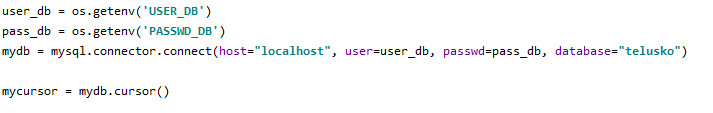
\includegraphics[scale=0.8]{conexionBD}
    \caption{Conexión desde Python con MySQL.}
    \label{fig:my_label}
\end{figure}
\imagen{conexionBD}{Conexión desde Python con MySQL.}

Realizadas todas las conexiones necesarias, se comenzó a buscar sobre librerías de sentiment analysis y como sería su integración con el proyecto.

Mientras, se escogió el template para angular y se ajustó a la aplicación. Después se eligió el segundo template, el de gráficos y se integró con el resto de la aplicación.

\imagen{manual_usuario/inicioES}{Página de inicio de la aplicación.}

Tras haber realizado los métodos de cálculo de análisis, se realizaron los cálculos estádisticos para almacenarlos en una nueva tabla en la base de datos.

\imagen{manual_usuario/tablaEstadisticasES}{Cálculos estadísticos.}

Teniendo ya la parte back end con los cálculos realizados y el front end con los templates bien integrados se comenzó a implementar varias funcionalidades como la de login o la del registro, y una de las principales, la visualización de los resultados en gráficos. 

\imagen{graficosR}{Gráficos implementados.}

Para ello fue necesario aprender a realizar peticiones desde la interfaz al servidor y saber formar el json correctamente en el servidor para que la información enviada fuera accesible.

\imagen{serviciotw}{Servicio de twitter.}
\begin{figure}[h]
    \centering
    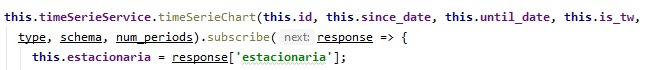
\includegraphics[scale=0.6]{response}
    \caption{Acceso a la información enviada del servidor a la interfaz.}
    \label{fig:my_label}
\end{figure}
\newpage
Además, se implementó la posibilidad de elegir entre qué fechas se quieren mostrar los resultados.
\begin{figure}[!h]
    \centering
    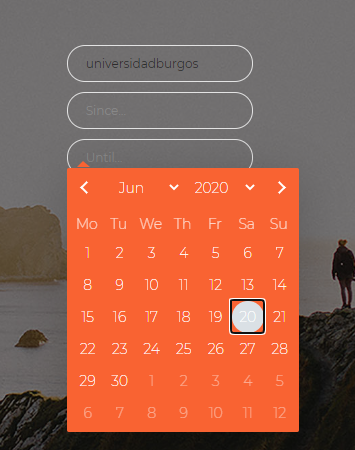
\includegraphics[scale=0.6]{manual_usuario/selectDate}
    \caption{Filtrar por fecha.}
    \label{fig:my_label}
\end{figure}
\FloatBarrier
Hasta el momento los resultados que se podían mostrar estaban previamente guardados, por lo que se añadió la opción de que aunque el identificador buscado no se encuentre en base de datos se busque en las APIs, se guarde en base de datos y se muestren los resultados.
\begin{figure}[h]
    \centering
    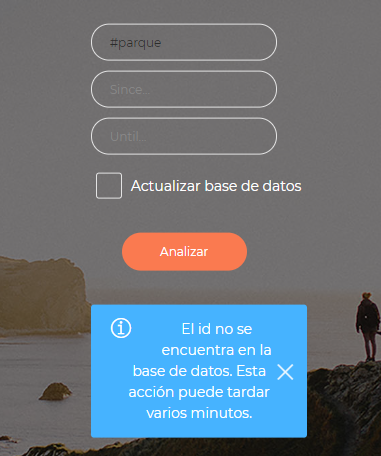
\includegraphics[scale=0.55]{manual_usuario/noIDES}
    \caption{Funcionalidad para buscar un id que no está en la base de datos.}
    \label{fig:my_label}
\end{figure}
\FloatBarrier

Además se añadió la opción de actualizar los identificadores que ya se encuentra en la base de datos.
\begin{figure}[h]
    \centering
    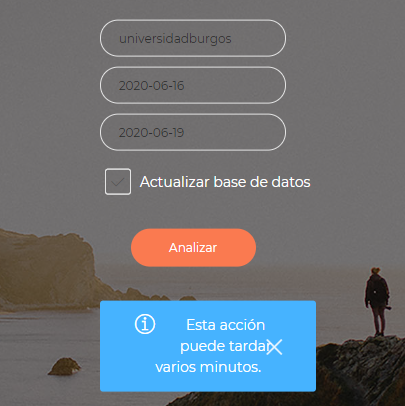
\includegraphics[scale=0.6]{manual_usuario/updateBDES}
    \caption{Funcionalidad para actualizar base de datos.}
    \label{fig:my_label}
\end{figure}
\FloatBarrier

En cuanto a la parte de desarrollo, lo último ha sido la funcionalidad de calcular y mostrar series temporales.

\imagen{manual_usuario/menuTSES}{Menú de elección para el cálculo de series temporales.}

\imagen{manual_usuario/TSgraficoES}{Gráfica de series temporales.}

La última implementación que se ha hecho ha sido la internacionalización, para la cual se han creado dos archivos de extensión json con las traducciones, unas en español y las otras en inglés.
\begin{figure}[h]
    \centering
    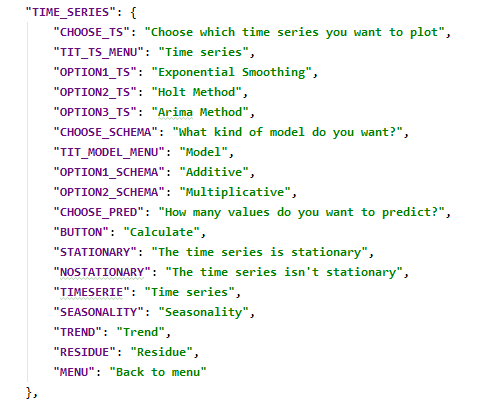
\includegraphics[scale=0.8]{internacionalizacion}
    \caption{Archivo json con las traducciones al inglés.}
    \label{fig:my_label}
\end{figure}

Todas estas implementaciones se han complementado con la documentación sobre el proyecto en memoria y anexos.

\subsection{Resolución de problemas técnicos}
Ha habido algunos problemas a lo largo del desarrollo del proyecto, que se han solventado con éxito.

\subsubsection{Problemas con Angular}

La mayoría de los problemas que se han tenido han sido con Angular ya que es un framework que nunca se había utilizado.

El primer problema fue conseguir ajustar el template de gráficos al template de angular que se ha utilizado para el resto de ventanas. 
Había varios conflictos entre los módulos ya que las versiones no coincidían. Además, algunas de las últimas versiones no son soportadas por estos templates por lo que daba varios errores y no se conseguía levantar la interfaz de usuario.

Ya conseguida la unión de los templates, hubo que aprender a crear servicios y enviar peticiones al servidor y desde este mandar un objeto json bien formado.
Para ello fueron muy útiles los ejemplos con pasos a seguir de la web de Angular como se ha comentado anteriormente.

Para la creación de los gráficos, ha sido necesario añadir un tiempo de parada entre los distintos servicios porque se solapaban entre ellos lo que resultaba en una petición de datos fallida con un código de error 500.

\subsubsection{Problemas con series temporales}
Inicialmente las series temporales a calcular iban a ser el suavizado exponencial, método de Holt y método de Holt-Winters.

Para realizar los cálculos de series temporales es necesario un periodo, el nuestro ha tenido que ser 1 ya que los datos se recogen y almacenan basándonos en el día en el que se crearon. Por ello, los periodos que tendrían sentido serían el 1 o el 7. 
Por ello, se creó un desplegable para que el usuario pudiera escoger entre los dos valores. Pero, al realizar cálculos con el periodo 7 la descomposición de la serie temporal no se realizaba correctamente en ningún caso, por lo que se optó por tener un periodo de 1 siempre.

El problema de tener este valor como periodo, es que el método de Holt-Winters no se podía calcular ya que al ser los valores de análisis tan pequeños, se generaban valores no reales que no se podían representar.
Por ello, decidimos eliminar esta serie temporal.

Pero en su lugar implementamos el modelo Arima, el cual es mucho más complejo y nos permite realizar predicciones más reales.

\subsubsection{Problemas con Heroku}

Para la presentación de la aplicación se decidió desplegar en Heroku, que es un hosting gratuito donde se puede alojar tu página web.
Hubo varios problemas desde el principio ya que el proyecto tiene dos partes, la parte del servidor en la que se realizan todas las operaciones y la interfaz de usuario.
Como están escritas en diferentes lenguajes fue necesario separar las partes para que Heroku pudiera reconocer ambas.
Tras conseguir esto, hubo que modificar algunas partes del código, como las URLs a las que se envían las peticiones, ya que apuntaban al Localhost y ya no iba a corresponder.

Cuando se realizaron las pruebas para ver que todo funcionaba correctamente, se notó la lentitud de la aplicación, pero al ser un hosting gratuito es normal ya que no nos ofrecen mucha memoria.

La aplicación funciona, pero al tener tantos servicios con peticiones agotamos la memoria RAM que nos ofrece Heroku y el rendimiento de la aplicación no es el esperado.

Para poder tener un buen rendimiento, sería necesario pagar una licencia que podría ascender a 250\EUR{}.

Por ello se ha optado por crear una máquina virtual en la que el tribunal pueda realizar las pruebas que considere con un rendimiento óptimo.

\subsubsection{Problemas con la máquina virtual}

Como se ha indicado en el apartado anterior, se ha considerado presentar el proyecto tanto en heroku como en una máquina virtual.
Inicialmente se creó una de Ubuntu, pero al empezar a instalar las dependencias se hizo imposible ya que daban fallos.

Se siguió con una Windows 7, la cual no nos permitió tampoco ya que indicaba que el sistema operativo estaba desactualizado para la version de Visual C++ Tools, las cuales son necesarias para las librerías de análisis de Python.

Por lo cual la solución ha sido comprar una licencia OEM Windows 10 Pro. Con esta se ha conseguido instalar todas las dependencias sin problema y tener la máquina virtual operativa.

Si no se ejecuta la máquina virtual en un ordenador lo suficientemente potente la aplicación puede sufrir fallos de llenado de memoria RAM, como sucedía en Heroku.
\capitulo{6}{Trabajos relacionados}

En este apartado vamos a ver varias herramientas que hacen uso del sentiment analysis.

\section{MonkeyLearn}
MonkeyLearn \cite{monkeylearn} es una aplicación que utiliza machine learning para analizar el texto. Puede integrarse con aplicaciones como Excel, Google Sheets, Zapier, Gmail, Twitter, etc. 

Además de poder utilizar su analizador de texto, te permite entrenarlo de forma personalizada añadiendo palabras que quieras destacar.

Respecto al precio, tiene tres planes diferentes:
\begin{itemize}
	
\item Un plan gratuito que está bastante reducido ya que te permite analizar 300 veces al mes, a baja velocidad y además no te permite ver los resultados en gráficos.
\item Un plan llamado “Team” que permite analizar hasta 10000 veces al mes con una velocidad media, se pueden definir hasta 3000 palabras nuevas para entrenar el algoritmo, pero tampoco nos permite mostrar los resultados en gráficos.
El precio es de 299\$ por mes.
\item Un plan llamado “Business” que es personalizado, nosotros nos encargaremos de decidir cuántas querys queremos analizar al mes, la velocidad de la aplicación, las palabras a definir. Además, los resultados se mostrarán en gráficos y flujogramas. 
El precio será variable.
\end{itemize}

\imagen{trabajos_relacionados/monkeylearn1}{Monkeylearn connect your text data.}

\imagen{trabajos_relacionados/monkeylearn2}{Monkeylearn turn your text into tags.}

\imagen{trabajos_relacionados/monkeylearn3}{Monkeylearn put your tags to work.}

\section{Lexalytics}
Es una aplicación que se basa en el Natural Language Processing para crear distintas librerías y modelos. Lexalytics \cite{lexalytics} también utiliza machine learning para entrenar a los modelos.

Además de utilizar sentiment analysis en los textos, los separan en categorías dependiendo del tema que se trate en el texto y extraen las distintas entidades como la persona que ha escrito, el lugar desde donde se escribe, los productos sobre los que se escriben, etc.

El precio de la aplicación es variable dependiendo de cuántos textos queramos analizar, el tiempo que vayamos a suscribirnos, etc. 

\begin{figure}[h]
    \advance\leftskip4cm 
    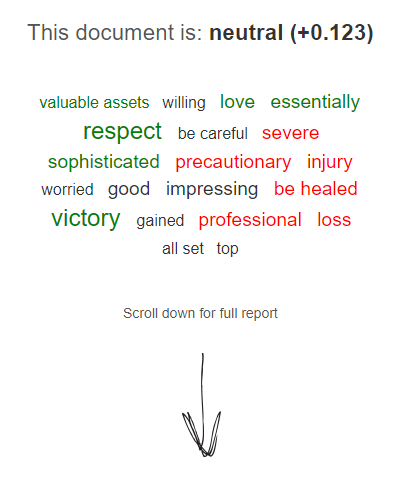
\includegraphics[scale=0.55]{trabajos_relacionados/lexalytics}
    \caption{Lexalytics análisis de texto}
\end{figure}


\imagen{trabajos_relacionados/lexalytics2}{Lexalytics entidades.}
\imagen{trabajos_relacionados/lexalytics3}{Lexalytics entidades subrayadas en el texto.}
\newpage
\section{Brandwatch}
Brandwatch \cite{brandwatch} es una aplicación que permite a las marcas saber que opina la gente sobre ellas en las redes sociales e internet mediante inteligencia artificial. 

Permite categorizar los datos y entrenar el modelo de forma personalizada añadiendo palabras que queramos que identifique como positivas o negativas en caso de estar en algún comentario.
Permite mostrar los datos recogidos en distintos tipos de gráficos y pudiendo personalizarlos para que muestre las categorías que queramos.

Además, nos permite analizar distintos perfiles de personas para poder realizar campañas de marketing que lleguen a las personas que queramos enfocar nuestra empresa.	

Los precios varían dependiendo de los planes:


\begin{table}[ht!]
    \centering
    \resizebox{15cm}{!} {
    \begin{tabular}{l l c}
    
         \textbf{Plan}    &\textbf{Descripción} &  \textbf{Precio } \\ \hline
         \textit{Brandwatch/Pro} &{Está orientado a analistas de marcas pequeñas}      & 653,59\$/mes \\ 
         \textit{Enterprise/M} &\parbox[p][0.2\textwidth][c]{8cm}{Para empresas de marcas algo más conocidas y por tanto con mayor volumen de opiniones}      & 2614,37\$/mes \\ 
         \textit{Enterprise/Q} &\parbox[p][0.2\textwidth][c]{8cm}{Orientado a empresas importantes y que tienen muchos comentarios que analizar}      & 2614,37\$/mes \\ 
    \end{tabular}}
    \caption{Precios de Brandwatch.}
    \label{tab:my_label}
\end{table}


Además cuentan con planes personalizados para agencias.

\imagen{trabajos_relacionados/brandwatch}{Brandwatch gráfico de líneas.}
\imagen{trabajos_relacionados/brandwatch2}{Brandwatch gráfico de burbujas.}

\capitulo{7}{Conclusiones y Líneas de trabajo futuras}

\section{Conclusiones}
Una vez finalizado el proyecto  y remontándome al comienzo del mismo puedo afirmar que he adquirido muchos conocimientos.

El resultado de la aplicación cumple con todos los objetivos marcados inicialmente y además se han añadido implementaciones que no se pensaron en un primer momento pero que dan al proyecto mayor funcionalidad.

Por ejemplo, en un primer momento se pensó que la aplicación simplemente iba a obtener los resultados que estuvieran en la base de datos ya almacenados. Pero a mitad del proyecto se pensó que podía ser muy interesante tener una opción de 'Actualizar la base de datos' y también la opción de buscar un identificador que no se encontrara almacenado.
De esta forma, nuestra aplicación accede a las APIs de Twitter e Instagram en tiempo real y recolecta datos nuevos para almacenarlos en la base de datos.

He aprendido mucho sobre las aplicaciones web, los protocolos utilizados y las peticiones a través de ellos. En cuanto a los lenguajes, he reforzado los conocimientos que tenía sobre Python y SQL, ya que se cursan a lo largo del grado, y he aprendido el lenguaje TypeScript. También he aprendido sobre HTML, sobre el cual tenía unos conocimientos muy vagos.

Personalmente, lo que más me ha costado y creo que he aprendido mucho, ha sido cómo conectar la interfaz de usuario de una aplicación con el controlador de la misma. Para mí utilizar servicios y realizar peticiones era algo totalmente nuevo, pero al final he conseguido aprender, y aunque me queda mucho por mejorar, he conseguido realizar las peticiones de forma exitosa.

En cuanto a las metodologías, las cuales se tratan en la asignatura de gestión de proyectos, se ha usado Scrum que actualmente está muy presente en la mayoría de los trabajos. Utilizarla ha sido clave para conseguir una buena organización y aprender a estimar cuanto tiempo gastamos en cada tarea.

Por todo ello, creo que el balance ha sido bueno aun con los problemas que se han tenido durante el desarrollo del proyecto.

\section{Líneas de trabajo futuras}

\begin{itemize}
    \item Crear varios roles de usuario.
    \item Implementar el acceso con cuentas de otras aplicaciones como Google, Facebook, etc.
    \item Implementar seguridad en la aplicación.
    \item Realizar sentiment analysis mediante técnicas de machine learning.
    \item Añadir más redes sociales de las que recabar información.
    \item Utilizar scraping para obtener información.
\end{itemize}


\bibliographystyle{plain}
\bibliography{bibliografia}

\end{document}
